% 第2章正文，根据《一二章.md》更新。
\FloatBarrier\clearpage

\section{作品设计与实现}\label{chapter:2}

\subsection{系统总体设计}\label{section:2.1}

\subsubsection{设计目标与系统总体架构}\label{section:2.1.1}

个人认知体检不仅需要记录用户浏览了多长时间，更需要了解这些时间里实际接触了哪些观点、获得了多少新的事实依据，以及是否反复接触通过不合理推断强化负面情绪的内容。由于短视频和社交平台中的信息分散出现，单独分析某条视频或某一天的浏览数量，难以反映信息重复与观点集中是否长期持续。因此，破茧以用户实际接触的内容和浏览事件为基础，将当前内容理解、个人历史比较与长期统计连接起来，形成能够持续更新的认知体检过程。

围绕这一目标，系统采用\textbf{手机授权采集、云端可信分析、加密历史存储与个人报告展示}相结合的总体架构。手机客户端负责获取用户授权范围内的屏幕及可采集音频，记录内容接触时间，并管理计算授权和长期密钥；云端可信计算环境负责将多模态内容转化为可比较的观点与论据，完成信息茧房和情绪引导分析；加密存储保存个人历史语义记录及统计结果，供后续浏览事件在授权后继续使用。各功能环节的职责与数据关系如表~\ref{tab:2-1}所示。

\begingroup
\small
\begin{longtable}{@{}
>{\RaggedRight\arraybackslash}p{(\linewidth - 6\tabcolsep) * \real{0.1600}}
>{\RaggedRight\arraybackslash}p{(\linewidth - 6\tabcolsep) * \real{0.2800}}
>{\RaggedRight\arraybackslash}p{(\linewidth - 6\tabcolsep) * \real{0.2900}}
>{\RaggedRight\arraybackslash}p{(\linewidth - 6\tabcolsep) * \real{0.2700}}@{}}
\caption{破茧系统主要功能环节及数据关系}\label{tab:2-1}\tabularnewline
\toprule
功能环节 & 需要解决的问题 & 核心处理 & 向后续环节提供的结果 \\
\midrule
\endfirsthead
\toprule
功能环节 & 需要解决的问题 & 核心处理 & 向后续环节提供的结果 \\
\midrule
\endhead
\bottomrule
\endlastfoot
授权采集与浏览记录 & 用户实际接触了什么内容、何时接触及停留多久 & 屏幕采样与区域裁剪、授权音频采集、浏览事件记录、加密上传 & 内容数据、接触时间、有效浏览时长与来源信息 \\
可信内容解析 & 不同形式的内容如何转化为统一的分析对象 & OCR、语音转写、文本对齐、议题与观点论据提取 & 带有原文位置的议题、观点、事实要点及论证关系 \\
个人认知分析 & 当前内容是否重复历史依据，是否存在过度推断型情绪引导 & 同议题历史比较、信息增量计算、多专家联合判别 & 观点分布、论据增量、情绪引导标签及其核验依据 \\
报告与交互服务 & 如何使长期分析结果便于理解、回顾和核查 & 按时段和议题汇总、长期风险预警、主题观点整理 & 小时、每日与长期认知体检报告，以及关联原文的提醒 \\
\end{longtable}
\endgroup

这些环节按浏览过程持续运行，其中观点和论据记录是两项认知分析任务的共同基础，浏览事件则负责把内容特征与用户实际接触情况联系起来。隐私保护并非在分析完成后附加的一项功能，而是贯穿手机采集、数据传输、模型推理和历史读写的运行约束，使上述处理能够在受保护的条件下持续开展。

\begin{figure}[htbp]
\centering
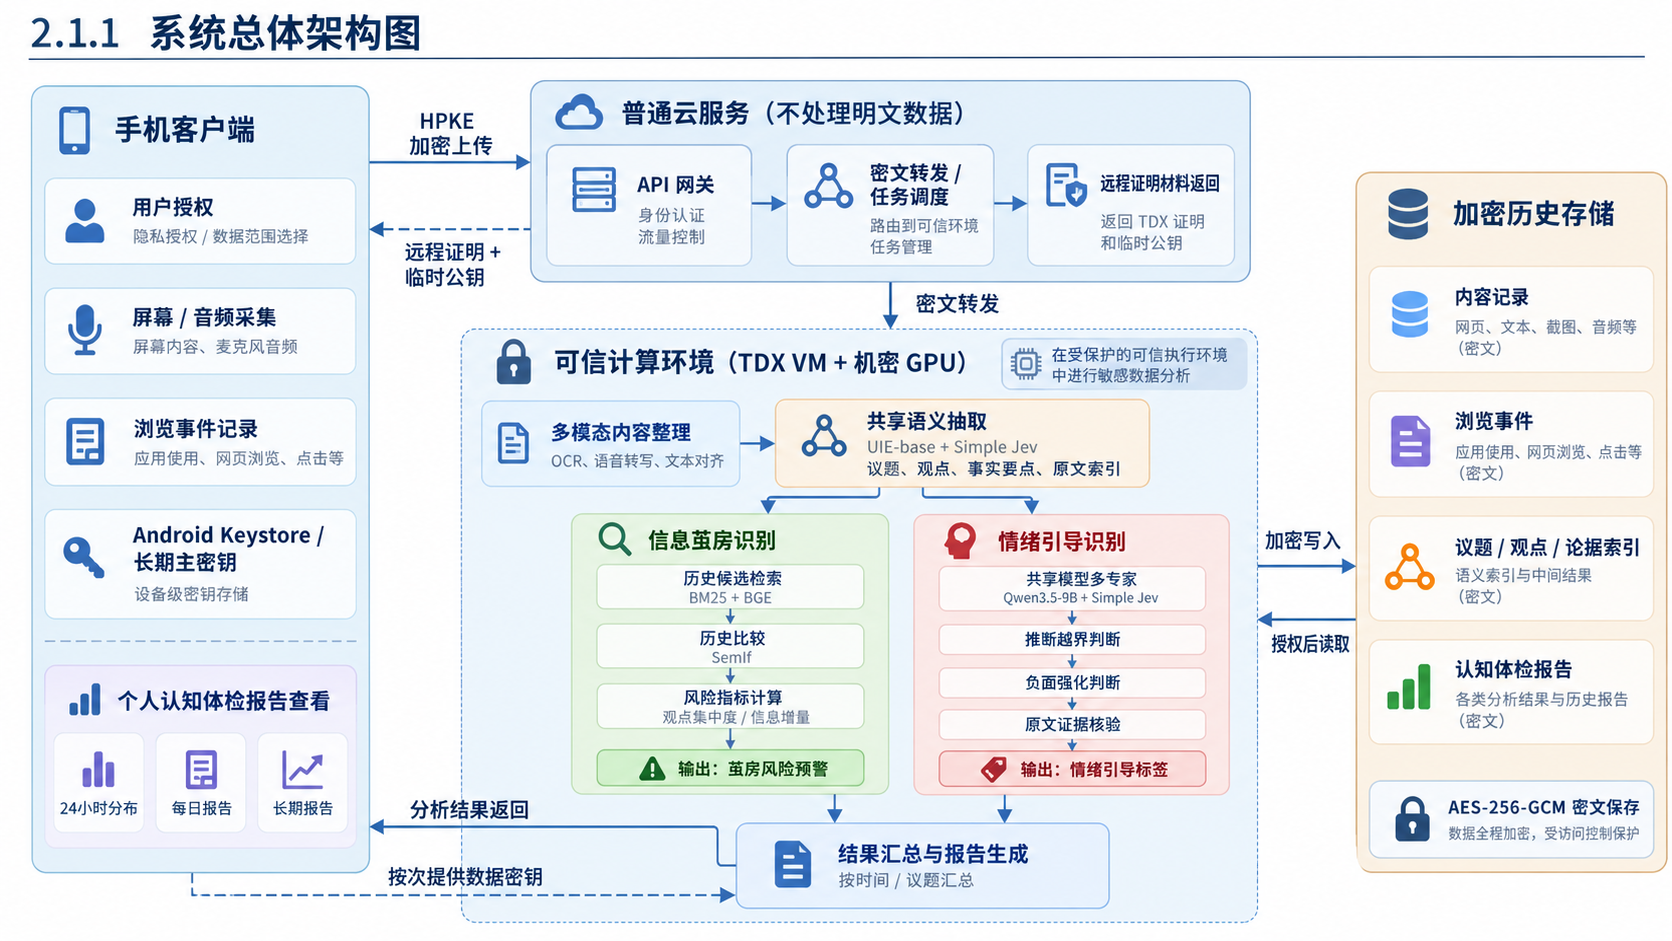
\includegraphics[width=\linewidth,height=0.72\textheight,keepaspectratio]{figures/chapter2/fig_2_1_system_architecture.png}
\caption{可信计算环境系统总体架构图}\label{fig:2-1}
\end{figure}

\subsubsection{多模态浏览内容采集与统一记录}\label{section:2.1.2}

网页、图文帖子和短视频的信息承载方式不同，同一观点可能出现在页面正文、视频字幕或口播中。若只采集某一种文本来源，便可能遗漏用户真正接触的事实与结论。针对这一问题，手机客户端在用户授权后通过Android MediaProjection获取屏幕内容，按照采样与区域裁剪规则保留可观察的信息，并在系统许可的条件下采集音频。同时记录相关内容的接触时间和有效浏览时长，为后续统计提供行为依据。

采集到的画面和音频经加密送入经过验证的可信计算环境，在其中完成OCR识别、语音转写以及文本顺序整理。系统依据页面结构、时间戳和可识别的内容来源，将文字、字幕与口播整理为具有上下文关系的文本片段，合并重复表达，并保留原文位置。这样，后续模型既能获得完整的语境，也能把识别结果追溯到具体页面区域、语句或视频时间点。

在数据组织上，系统区分\textbf{内容记录}与\textbf{浏览事件}。内容记录保存某条内容的可分析文本、来源和原文索引；浏览事件保存用户每次接触该内容的时间及有效停留信息。同一内容未发生变化而被反复观看时，系统可以复用既有的内容解析结果，但仍分别记录每次接触。由此，观点与论据分析以内容为对象，出现频率和浏览时长统计以事件为对象，避免把同一内容的重复观看误认为不同事实，也避免遗漏重复接触本身所反映的信息环境特征。

\subsubsection{共享语义抽取与双路径认知分析}\label{section:2.1.3}

完成多模态文本整理后，系统首先需要回答一条内容究竟讨论了什么问题，表达了哪些判断，以及使用了什么事实加以支持。只有将这些内容转化为稳定的语义记录，才能比较不同视频之间的信息差异，也才能检查负面结论是否超出了原有事实。为此，系统采用2.2节提出的轻量化观点论据提取方法：通过UIE-base定位议题、观点、事实片段及限定条件，再由基于Qwen3.5-0.8B的Simple Jev判别表达类型和观点---论据关系，并将复合论据整理为可独立比较的事实要点。提取结果保留原文位置，供后续两条分析路径共同使用。

\textbf{第一条路径面向信息茧房识别，重点判断当前内容相对于个人历史增加了什么。} 系统利用BM25与BGE-small-zh-v1.5检索相近议题及历史语义候选，再由基于Qwen3.5-4B的SemIf判断议题归属、观点关系和事实等价性。在确定所属议题后，当前论据与该议题下的历史事实要点进行比较，综合不同历史记录的覆盖情况，识别已出现的依据和新增信息。系统进一步按照议题及时间窗口计算观点集中度、有效观点数量、去重论据数量和信息增量率，在有效记录达到要求后，考察主导观点持续集中且新增依据持续不足的情况，并将相关浏览记录作为风险预警的依据。

\textbf{第二条路径面向过度推断型情绪引导识别，重点判断内容如何从事实推导出负面结论。} 系统复用前述事实、观点和论证关系，以整条内容为上下文、以具体评价性结论为判别单元。基于Qwen3.5-9B与Simple Jev的共享模型多专家方法，分别识别事实适用范围的不合理扩大、结论确定程度的提高，以及灾难化或无助化等负面情绪强化。只有推断越界与负面强化同时成立，且能够通过原文证据核验时，才将相应内容标记为过度推断型情绪引导。随后将识别结果与浏览事件关联，统计此类内容的接触次数和有效浏览时长。

两条路径共享内容解析结果和原文证据索引，但分别回答``是否持续获得新的判断依据''和``所接触的结论是否通过不合理推断强化负面情绪''两个问题。系统将它们的结果按照时间和议题汇总，生成24小时信息分布、每日报告和长期分析报告。用户不仅可以查看不同观点的接触比例、信息增量与情绪引导内容占比，还可以进入具体议题，回顾支持各类观点的已浏览内容及其主要论据。对于观点长期集中或依据持续重复的议题，报告提供风险提醒和信息覆盖局限提示，并保留相关原始来源，供用户进一步核查和补充资料。

\paragraph{端侧脱敏与云端结构化接口协同模式的工程边界}
复赛工程在现有服务端保留兼容路由，并增加端侧脱敏的结构化API协同路径。手机在上传前对手机号、身份证号、电子邮箱及识别到的通知前缀执行本地掩码，携带至多15条历史事实候选；模型单次输出观点、事实覆盖关系、情绪引导证据及信息盲区，程序再检查JSON类型、历史引用、事实计数和连续原文片段。有限候选下的历史覆盖不等同于全量历史穷尽核验，正则掩码也不等同于完全匿名化。

该路径采用固定Ed25519公钥验证应用代码度量声明，以X25519和HKDF-SHA256派生双向AES-256-GCM会话密钥，结合持久化版本、哈希及手机检查点检查状态连续性。这是应用层身份与完整性机制，不构成下文硬件TEE远程证明的等价实现。服务进程及所调用的商业模型能够处理脱敏明文，不能据此宣称云端全程不可见明文。本文原有本地模型与硬件隔离设计作为研究方案保留，其实验结论不直接迁移为此API路径的准确率、时延或机密性结论；新增路径的现场可用性需单独验收。

\subsubsection{高频处理与长期历史维护}\label{section:2.1.4}

短视频信息流的内容切换频繁，若每出现一条新内容都由大模型生成完整解释，再逐项扫描全部历史记录，分析任务便容易积压，影响连续体检的使用体验。破茧因此将高频处理拆分为\textbf{片段定位、固定类别判断、历史候选检索和指标计算}四类任务，让不同计算需求由适合的技术承担。

在当前内容处理阶段，UIE-base负责定位语义片段，Simple Jev通过候选类别评分完成结构化判断，减少长文本生成；情绪引导识别中的三个专家共享Qwen3.5-9B的内容上下文，降低重复输入带来的推理开销。在历史比较阶段，BM25与语义检索先缩小候选范围，SemIf只针对相关议题、观点和论据执行关系判别；观点分布、信息新颖度与风险条件则由确定性程序计算。对于内容未发生变化的重复接触，系统复用相应的抽取与判别结果，只为新的浏览事件增加接触记录。

计算提速还必须与历史结果的正确性相协调。不同内容的OCR、文本整理和初步语义抽取可以独立处理；同一用户的历史覆盖判断与语义状态更新则按照实际浏览顺序执行，或依据明确的历史版本完成计算。随着新内容增加，系统按议题持续维护观点簇、事实要点和检索索引；当后续比较确认两个议题或观点簇需要合并时，同步修正历史关联，并重新计算受影响的增量与统计结果。这样，系统能够利用并行处理和历史结果复用适应高频浏览需求，同时保持长期分析口径的一致性。

\subsubsection{贯穿全过程的隐私保护机制}\label{section:2.1.5}

持续认知体检必须长期比较用户浏览历史，而议题、观点、论据和情绪统计等记录本身也可能揭示个人关注的敏感问题。即使原始截图不作长期保存，如果历史索引或分析报告能够被普通服务器管理者读取，仍会带来隐私泄露风险。因此，破茧按照2.4节提出的可验证异构机密计算方案，围绕\textbf{采集端程序可信、上传对象可信、运行中明文受保护、历史解密权由用户控制}建立连续防护链路。

在手机端，系统通过公开安全关键代码、可复现构建及发布版本审核约束采集与对外通信行为。上传数据之前，客户端核验云端Intel TDX可信虚拟机、NVIDIA机密GPU及已批准程序版本的远程证明，并检查本次接收公钥与证明的绑定关系。核验通过后，手机才使用HPKE加密提交数据；普通业务网关仅负责转发密文。真正的解密发生在受保护的CPU内存中，随后的OCR、语音转写、语义模型推理及历史比较均位于经过验证的可信计算边界内，涉及GPU的处理使用受保护的显存与通信链路。

对于需要长期保存的浏览事件、语义索引和认知体检报告，系统使用AES-256-GCM加密存储，并将长期主密钥保留在受Android Keystore保护的手机端。每次需要读取个人历史时，客户端重新验证可信程序，只按次交付本次所需的数据密钥；可信程序在内部完成解密、分析、更新及重新加密，并通过历史版本标识检查状态连续性。分析报告以密文形式保存，或经受保护会话返回手机供用户查看。由此，普通服务器能够管理任务和密文存储，却不能仅凭运维权限获得浏览原文或长期分析结果的解密权。

通过上述设计，破茧形成以真实浏览事件为入口、以观点论据记录为共同基础、以长期历史比较和情绪引导判别为核心的认知体检系统。2.2节进一步介绍观点与论据增量识别及信息茧房风险判定，2.3节介绍共享模型多专家情绪引导识别，2.4节说明各处理阶段如何在可验证的可信计算条件下保护个人隐私。

\subsection{基于观点与论据历史增量的信息茧房识别方法}\label{section:2.2}

\subsubsection{研究问题与总体技术思路}\label{section:2.2.1}

仅凭用户浏览主题的集中程度，无法准确判断其是否陷入信息茧房。例如两名用户都在关注就业形势：一人持续阅读不同地区的招聘数据、行业报告和相互补充的分析；另一人则反复看到不同账号转述同一份报告，并不断重复阅读着相似的结论。两者的浏览主题同样集中，前者不断获得新的判断依据，后者接触的内容虽然数量增加，实际提供的信息却变化有限。因此，识别信息茧房需要考察同一\textbf{议题下的观点是否趋于单一，以及支撑这些观点的论据是否缺乏增量。}

针对这一问题，破茧采用\textbf{基于轻量化信息抽取的观点增量识别方法}。系统首先从用户实际浏览的网页、短视频和评论中提取议题、观点及其论据，再将当前语义内容与个人历史记录比较，识别重复依据和新增事实，最后依据一段时间内的观点分布与论据增量判断信息茧房风险。

为适应连续浏览场景中的高频分析需求，系统将原本由生成式大模型承担的语义处理拆分为两个阶段。在当前内容分析阶段，采用UIE-base定位观点与事实片段，利用基于Qwen3.5-0.8B的Simple Jev进行表达类型和论证关系判别；在历史比较阶段，利用BM25与BGE-small-zh-v1.5召回相关议题及历史语义候选，再由基于Qwen3.5-4B的SemIf完成议题匹配、观点归并与论据关系判别。两套本地决策框架均直接对预设选项评分，以降低单次判别的生成开销。事实覆盖、窗口指标和长期风险则由确定性程序计算，形成从当前内容理解到历史增量分析的连续处理链路。

流程图如图所示（后续改）：

\begin{figure}[htbp]
\centering
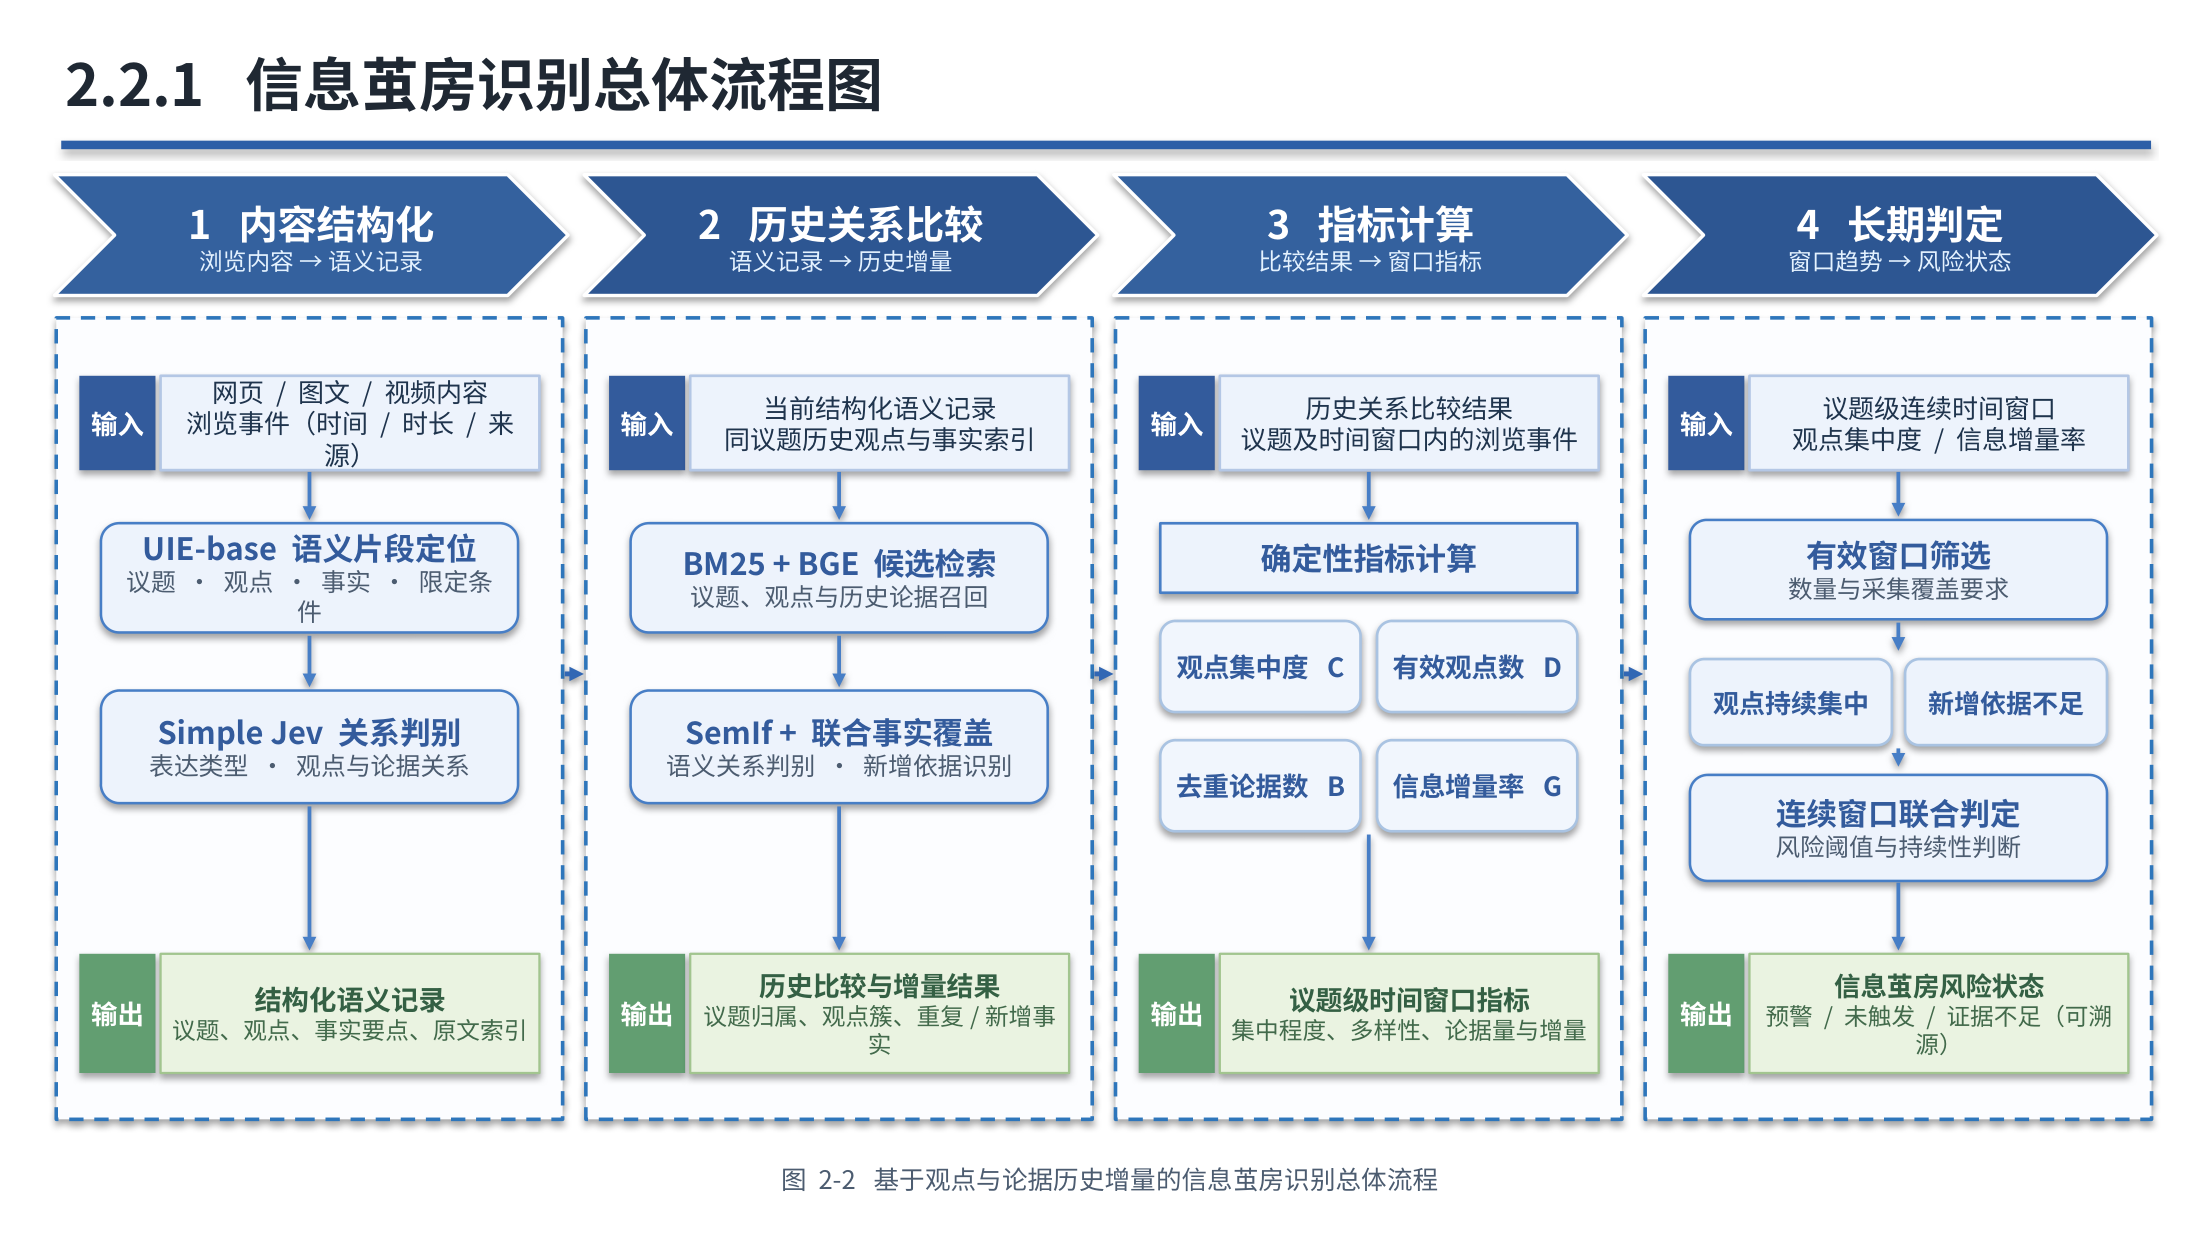
\includegraphics[width=\linewidth,height=0.72\textheight,keepaspectratio]{figures/chapter2/fig_2_2_cocoon_detection.png}
\caption{信息茧房识别总体流程图}\label{fig:2-2}
\end{figure}

\subsubsection{基于UIE与本地结构化决策的观点论据提取}\label{section:2.2.2}

判断信息是否重复，首先要明确一条内容实际表达了什么观点，又使用了哪些依据。网络文章和短视频常将事实、个人经历和主观判断交织在一起，同一段话还可能讨论多个问题。若直接比较整段内容，容易将观点相近但依据不同的材料判为重复，也可能忽略不同表达中反复引用的同一事实。因此，系统先定位原文中的语义片段，再识别片段类型及其论证关系。

系统将接收采集模块收集到的网页文字、OCR识别结果和语音转写文本，依据页面结构、时间戳和来源标识恢复可观察内容的顺序。预处理合并字幕与画面文字中的重复内容，按句子和段落组织文本，并保留必要的相邻上下文。对于较长的文章和视频，采用带重叠上下文的分段方式，每个片段均保存内容标识、原文位置、接触时间和可识别的表达主体，使后续抽取结果能够追溯到用户实际接触的内容。

在片段定位阶段，系统采用通用信息抽取模型UIE-base，按照预设的抽取模式识别议题表述、判断性语句、事实性片段，以及时间、地区、人群等限定条件。\textbf{观点}指针对某一问题提出的判断，例如``应届生求职竞争正在加剧''；\textbf{论据}指内容为支持或反驳某种判断而引用的事实、数据、案例或解释，例如``某地区互联网行业招聘岗位同比减少20\%''。UIE返回候选片段及其原文位置，为后续判断提供明确的文本对象。

语句片段在论证中的作用，需要结合上下文进一步判断。例如，文章可能先引用``就业形势正在好转''的说法，再提出反对意见；一项招聘数据也可能被作者用于支持多个判断。因此，系统将UIE提取的候选片段及局部上下文输入本地Simple Jev，由Qwen3.5-0.8B对预定义问题进行结构化决策。模型首先区分事实陈述、观点表达与引用内容，再针对候选观点---论据组合判断其关系属于支持、反驳、无关或不确定，并结合上下文确定表达主体。对于同一片段涉及的多个判别问题，采用共享上下文的批量决策方式返回类别及相应分值。

为支持后续的信息增量计算，系统进一步把包含多项独立事实的论据划分为事实要点。具体做法是利用句法边界、并列连接和UIE定位结果生成候选要点，再由Simple Jev判断其是否具有相对完整的事实含义，并确认主体、时间和适用范围。这样，一条同时讨论``招聘岗位减少''和``应聘人数增加''的论据可以保留两个独立要点。对于跨句表达，系统结合重叠上下文检查要点与原文的对应关系。

整理后的结果通过原文位置校验和字段一致性检查，写入统一的语义记录。对于第\(i\)次浏览涉及的议题\(q\)，记为\(z_i^q=(\mathcal V_i^q,\mathcal E_i^q,\mathcal R_i^q)\)，其中\(\mathcal V_i^q\)为观点集合，\(\mathcal E_i^q\)为带有事实条件和要点信息的论据集合，\(\mathcal R_i^q\)为观点与论据之间的论证关系。每项记录均保留原始来源和表达主体，作为后续历史比较及主题观点整理的共同输入。

\subsubsection{基于SemIf的历史语义比较与信息增量识别}\label{section:2.2.3}

一项事实是否属于新增信息，取决于用户此前已经接触过什么。系统将第\(i\)次接触记录为浏览事件\(b_i=(x_i,t_i,d_i)\)，分别表示浏览内容、接触时间和有效接触时长，并按议题维护历史观点与论据索引。新内容完成结构化提取后，依据实际浏览顺序与此前的历史进行比较，再写入本次记录。对于重复观看，系统复用已有的片段提取结果，同时保留新的接触事件，使内容计算与实际接触次数相互区分。

\begin{figure}[htbp]
\centering
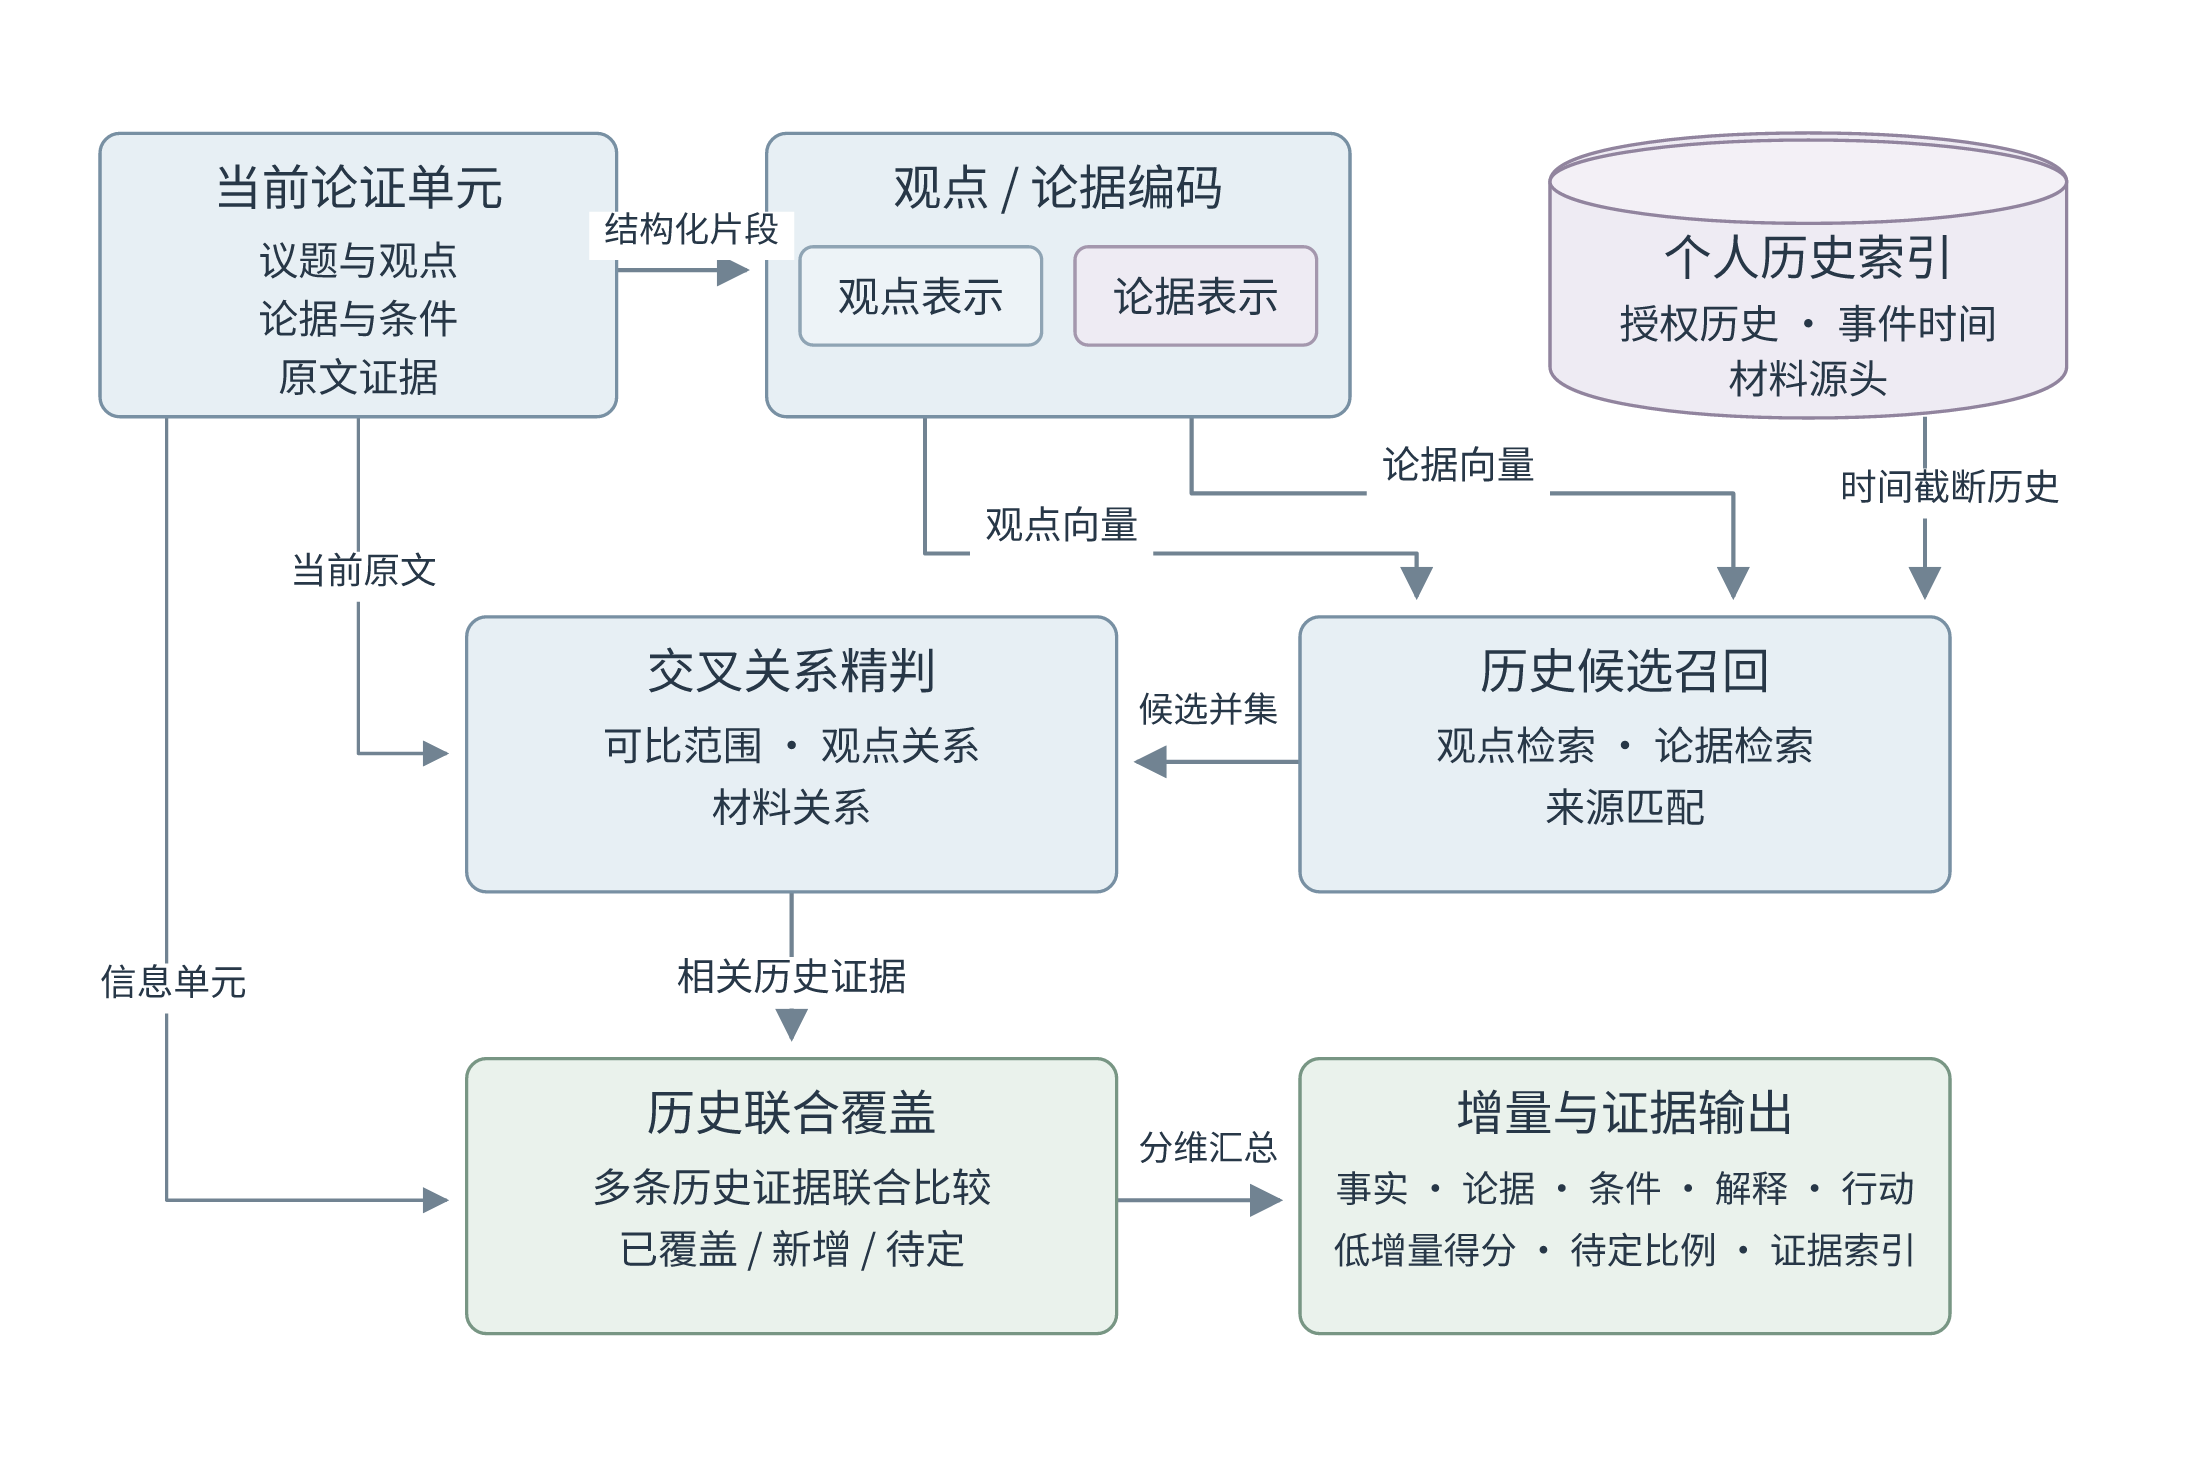
\includegraphics[width=\linewidth,height=0.72\textheight,keepaspectratio]{figures/chapter2/fig_2_3_history_increment.png}
\caption{分级匹配与历史更新流程图}\label{fig:2-3}
\end{figure}

在历史比较之前，系统先确定当前内容所属的议题。对于UIE提取的议题表述，利用BM25与BGE-small-zh-v1.5分别从词项和语义层面召回个人历史中的相近议题，再由SemIf判定同一议题、上下位相关或不同议题。判定为同一议题的内容归入已有档案，上下位议题保留关联；无法归入已有档案的内容建立新议题，并初始化观点簇与论据索引。

确定议题归属后，系统使用\textbf{观点与论据双路候选检索}：观点检索关注讨论对象与判断方向，结合BM25与BGE-small-zh-v1.5召回相近观点；论据检索关注事实主体、数据和适用条件，利用BM25召回候选，再依据结构化字段筛选和排序。由此将针对全部历史的比较，转化为当前语义单元与少量候选之间的关系判别。

对于检索得到的候选，系统采用\textbf{基于SemIf的本地语义关系决策方法}。SemIf以当前观点或论据、候选历史片段及其事实条件为共同输入，利用Qwen3.5-4B直接读取预设关系选项的模型分值。观点比较区分语义相近、相互反驳及不同判断；论据比较区分事实等价、部分重合、不同事实及无法确定，并重点检查主体、时间、地区等限定条件是否一致。对于同一当前语义单元召回的多项候选，复用共同输入上下文进行多项关系判断。

根据观点关系判别结果，系统将判断对象、方向及适用条件一致的观点归入已有簇，对无法归并的观点建立新簇，并保留不同观点簇之间的反驳关系。新议题和观点簇的展示名称优先采用UIE抽取的原文表述；缺少适合展示的名称时，复用Qwen3.5-4B的常规文本生成接口生成简明名称。议题和观点簇使用稳定标识存储，名称用于浏览报告中的展示。

单项候选比较仍无法完整反映历史信息的覆盖情况。一条新视频可能重新组合此前多条视频提供的事实，虽然没有任何一条历史材料与之完全一致，其中的事实却可能都已出现。因此，系统采用\textbf{基于事实要点的历史证据联合覆盖方法}：以2.2.2节形成的事实要点为单位，汇总来自不同历史记录的SemIf判别结果。只有当历史材料能够覆盖某一要点的事实内容及必要限定条件时，才将该要点认定为已出现；多个要点可以分别由不同历史来源覆盖。

设当前论据\(e\)包含\(J_e\)个事实要点，第\(j\)个要点的历史覆盖标记为\(c_j\)，已覆盖取1、新增取0。其历史覆盖程度定义为：

\begin{equation}
\operatorname{Cov}(e,\mathcal H_q^{<i})=\frac{\sum_{j=1}^{J_e}\omega_jc_j}{\sum_{j=1}^{J_e}\omega_j},\qquad c_j\in\{0,1\}
\label{eq:2-1}
\end{equation}

其中，\(\mathcal H_q^{<i}\)表示本次浏览发生前的同议题历史记录，\(\omega_j\)为事实要点权重，初始采用等权计算。在此基础上，定义当前论据相对于个人历史的信息新颖度：

\begin{equation}
\nu(e,\mathcal H_q^{<i})=1-\operatorname{Cov}(e,\mathcal H_q^{<i})
\label{eq:2-2}
\end{equation}

对于首次出现的议题，\(\mathcal H_q^{<i}\)为空，已识别的有效事实要点均计为新增；对于已有议题中新建的观点簇，论据仍与该议题的全部历史记录进行比较。

例如，一条视频同时提到``招聘岗位减少''\,``应聘人数增加''和一项新的毕业生调查结果。前两项分别出现在用户此前浏览过的不同视频中，第三项为首次接触的事实。在三个要点等权时，该论据的信息新颖度为\(1/3\)。系统保存每项覆盖判断所对应的历史片段和原始来源；对于尚不能确认覆盖关系的论据，先保留待核验状态，确认后再纳入有效增量统计。

随着浏览记录增加，系统复用候选检索与SemIf机制复核可能重合的议题和观点簇。确认属于同一议题或同一观点的簇进行合并，保留旧簇标识到目标簇的映射，并更新浏览事件关联及历史检索索引。对于议题归属发生变化的记录，按原始浏览顺序重新计算受影响的历史事实覆盖与窗口指标；观点簇合并则同步更新观点分布指标和相关风险结果。原文片段及其来源记录继续保留，供后续追溯。

由于不同内容的抽取可以独立执行，系统允许新浏览内容并行完成UIE与Simple Jev处理；涉及个人历史的语义比较和状态更新则按照浏览事件的实际顺序执行，或基于相应的历史版本进行计算。这样既能减少前端浏览对后台分析的等待，也能保证信息新颖度始终相对于正确的先前历史定义。

\subsubsection{观点分布与信息增量指标计算}\label{section:2.2.4}

完成观点归并和历史比较后，系统以\textbf{议题\(q\)和时间窗口\(W\)}为统计单位，将分散的浏览记录转化为四项指标。设\(\mathcal B_q(W)\)为窗口内与议题\(q\)相关的有效浏览事件集合，\(K_q\)为该窗口出现的观点簇数量。同一浏览事件对同一观点簇计一次，一条内容涉及不同观点时分别记录。四项指标分别反映观点接触的集中程度、分布多样性、依据数量和历史增量。

\textbf{（1）观点集中度。} 为衡量用户是否主要接触某一种判断，先计算第\(k\)个观点簇在窗口内的接触比例：

\begin{equation}
p_{qk}(W)=\frac{n_{qk}(W)}{\sum_{j=1}^{K_q}n_{qj}(W)}
\label{eq:2-3}
\end{equation}

其中，\(n_{qk}(W)\)为关联该观点簇的有效浏览事件数。在此基础上，以占比最高的观点衡量集中程度：

\begin{equation}
C_q(W)=\max_{1\leq k\leq K_q}p_{qk}(W)
\label{eq:2-4}
\end{equation}

\(C_q(W)\)越高，说明用户接触的内容越集中于某一主导观点。例如，围绕就业形势的有效观点接触中，若80\%表达``形势趋于严峻''，则观点集中度为0.8。

\textbf{（2）有效观点数量。} 观点集中度反映主导观点的优势。系统进一步采用基于信息熵的有效观点数量，刻画不同观点的整体分布：

\begin{equation}
D_q(W)=\exp\left(-\sum_{k=1}^{K_q}p_{qk}(W)\ln p_{qk}(W)\right)
\label{eq:2-5}
\end{equation}

当所有接触都集中于一个观点时，该指标为1；当多个观点的接触份额更加均衡时，指标相应增大。该指标与观点集中度共同呈现用户所接触观点的结构。

\textbf{（3）去重论据数量。} 同一事实可能被不同账号反复引用，仅统计论据出现次数会高估信息丰富度。系统依据SemIf得到的历史语义关系，对事实内容及适用条件一致的论据进行归并，计算窗口内实际涉及的不同依据数量：

\begin{equation}
B_q(W)=\left|\operatorname{Dedup}(\mathcal E_q(W))\right|
\label{eq:2-6}
\end{equation}

其中，\(\mathcal E_q(W)\)为窗口内的论据出现记录，\(\operatorname{Dedup}\)表示基于语义等价与事实条件的去重操作。例如，十条视频均引用同一项招聘调查时，该调查计为一项去重论据，各视频的出现次数与来源仍分别保留。

\textbf{（4）信息增量率。} 去重论据数量反映窗口内接触了多少种不同依据，信息增量率进一步衡量这些依据相对于此前历史增加了多少内容。设\(\mathcal E_{i,\mathrm{valid}}^q\)为第\(i\)次浏览中已完成历史覆盖判断的论据集合，则窗口信息增量率定义为：

\begin{equation}
G_q(W)=\frac{\displaystyle\sum_{b_i\in\mathcal B_q(W)}\sum_{e\in\mathcal E_{i,\mathrm{valid}}^q}\nu(e,\mathcal H_q^{<i})}{\displaystyle\sum_{b_i\in\mathcal B_q(W)}|\mathcal E_{i,\mathrm{valid}}^q|}
\label{eq:2-7}
\end{equation}

\(G_q(W)\)表示窗口内有效论据信息新颖度的平均值。数值较低说明当前浏览内容较多复用了已接触的事实，数值较高则说明用户持续获得新的判断依据。该指标与观点集中度结合，可以区分``观点相近但论据持续增加''和``观点相近且依据长期重复''两种不同的信息接触模式。没有有效论据的窗口不计算信息增量率，也不计入需要该指标的有效风险判定窗口。

\subsubsection{基于长期浏览记录的信息茧房风险判定}\label{section:2.2.5}

判断信息茧房的长期风险，需要考察观点集中与依据重复的持续性。例如，用户为准备求职面试连续观看多条相关视频，可能暂时形成较高的观点集中度。因此，系统按日或设定时长汇总观点分布与信息增量，重点考察\textbf{主导观点持续集中、同时新增论据持续不足}的接触模式。

设\(W_t\)为第\(t\)个时间窗口。当观点集中度达到阈值\(\theta_C\)，且信息增量率低于阈值\(\theta_G\)时，定义该窗口满足联合条件：

\begin{equation}
A_q(W_t)=\mathbb I\left[C_q(W_t)\geq\theta_C\ \land\ G_q(W_t)\leq\theta_G\right]
\label{eq:2-8}
\end{equation}

系统进一步记录联合条件连续成立的窗口数量。设\(U_q(W_t)\)为窗口有效性标记，\(\ell_q(t)\)为截至第\(t\)个窗口的连续长度，其更新规则为：

\begin{equation}
\ell_q(t)=\begin{cases}\ell_q(t-1)+1,&U_q(W_t)=1\ \land\ A_q(W_t)=1,\\0,&\text{其他情况。}\end{cases}\qquad \ell_q(0)=0
\label{eq:2-9}
\end{equation}

窗口有效性依据可用浏览数量、采集覆盖和已完成的语义分析结果确定。设观察期内的最大连续长度为\(L_q(T)=\max_{1\leq t\leq T}\ell_q(t)\)，有效窗口数量为\(n_q^{\mathrm{valid}}(T)\)。当有效记录达到最低数量要求，且联合条件持续达到设定长度时，系统输出信息茧房风险预警：

\begin{equation}
R_q(T)=\begin{cases}\bot,&n_q^{\mathrm{valid}}(T)<n_{\min},\\1,&L_q(T)\geq L_{\min},\\0,&\text{其他情况。}\end{cases}
\label{eq:2-10}
\end{equation}

其中，\(n_{\min}\)为最低有效窗口数，\(L_{\min}\)为持续性阈值；\(R_q(T)\)分别以1、0和\(\bot\)表示触发预警、未触发预警及证据不足。各阈值根据标注数据上的误报和漏报表现确定。预警结果同时关联对应的时间窗口、主导观点、重复论据及原始来源，使用户能够了解风险判断来自哪些实际浏览内容。

通过上述方法，破茧将浏览过程中的零散观点与论据转化为可追溯的长期信息接触特征。UIE与本地快速决策模型承担高频语义处理，SemIf完成个人历史关系判别，确定性程序计算观点结构和事实增量。\textbf{系统据此考察同一议题下观点的持续集中程度，以及支撑这些观点的事实依据是否仍在增加。}

\subsection{基于共享模型多专家判别的情绪引导识别方法}\label{section:2.3}

\subsubsection{研究问题与总体技术思路}\label{section:2.3.1}

在网络平台上，点击数量与用户互动往往直接影响内容的传播效果，部分内容创作者会刻意放大现实问题中的负面因素以博取更多互动与流量，例如通过制造焦虑、恐惧等情绪吸引用户持续评论与转发。这类内容通常并不直接编造虚假信息，而是通过个别的真实事件或有限数据为依据，将局部现象夸大为普遍趋势。例如，某家企业缩减招聘规模是真实事件，但据此断言``就业市场已经全面崩溃，普通人再努力也没有出路''，强化了受众对就业前景的焦虑。由于这类内容往往包含真实的事实依据，其引导性主要体现在从事实到结论的过度推断过程中存在逻辑问题，因此仅依靠虚假信息检测或情绪分类，难以准确识别其中的情绪引导。

针对这一问题，破茧重点识别\textbf{网络内容是否利用有限的事实依据，推导出夸大或绝对化的负面结论，从而强化受众的焦虑、恐惧等情绪}。判断过程需要同时回答三个相互关联的问题：原文提供了什么事实，事实能够支持多大范围的结论，以及评价性表达是否进一步强化了焦虑、恐惧或无助感。只有把这些判断与原文片段联系起来，系统才能给出可核查的情绪引导识别结果。

为完成这一判断，系统还需要解决网络内容中事实与结论分散的问题。一条短视频可能先介绍局部事件，再穿插其他材料，最后给出面向整体形势的评价；同一条内容也可能包含多个不同的结论。孤立分析某一句话，难以准确判断它与前文事实的关系。为此，系统复用2.2节抽取的事实、观点及论证关系，以\textbf{整条内容为分析上下文，以具体评价性结论为判别单元}，分别检验每项结论与其相关依据之间的关系。

日常信息流还具有内容出现频繁、浏览间隔短的特点。针对这一需求，破茧采用\textbf{Qwen3.5-9B与Simple Jev相结合的共享模型多专家判别方法}：由同一语言模型承担三个维度的语义判断，利用Simple Jev替代传统的LLM技术来加速该分析过程，先在共享上下文上完成预设类别的候选评分，然后再通过逻辑规则融合各项判断，最后在生成报告时利用2.2节保留的原文索引来还原原文内容。由此，系统将复杂的情绪引导分析转化为可复用的结构化判别过程，为连续浏览场景下的内容识别和接触统计提供基础。

\begin{figure}[htbp]
\centering
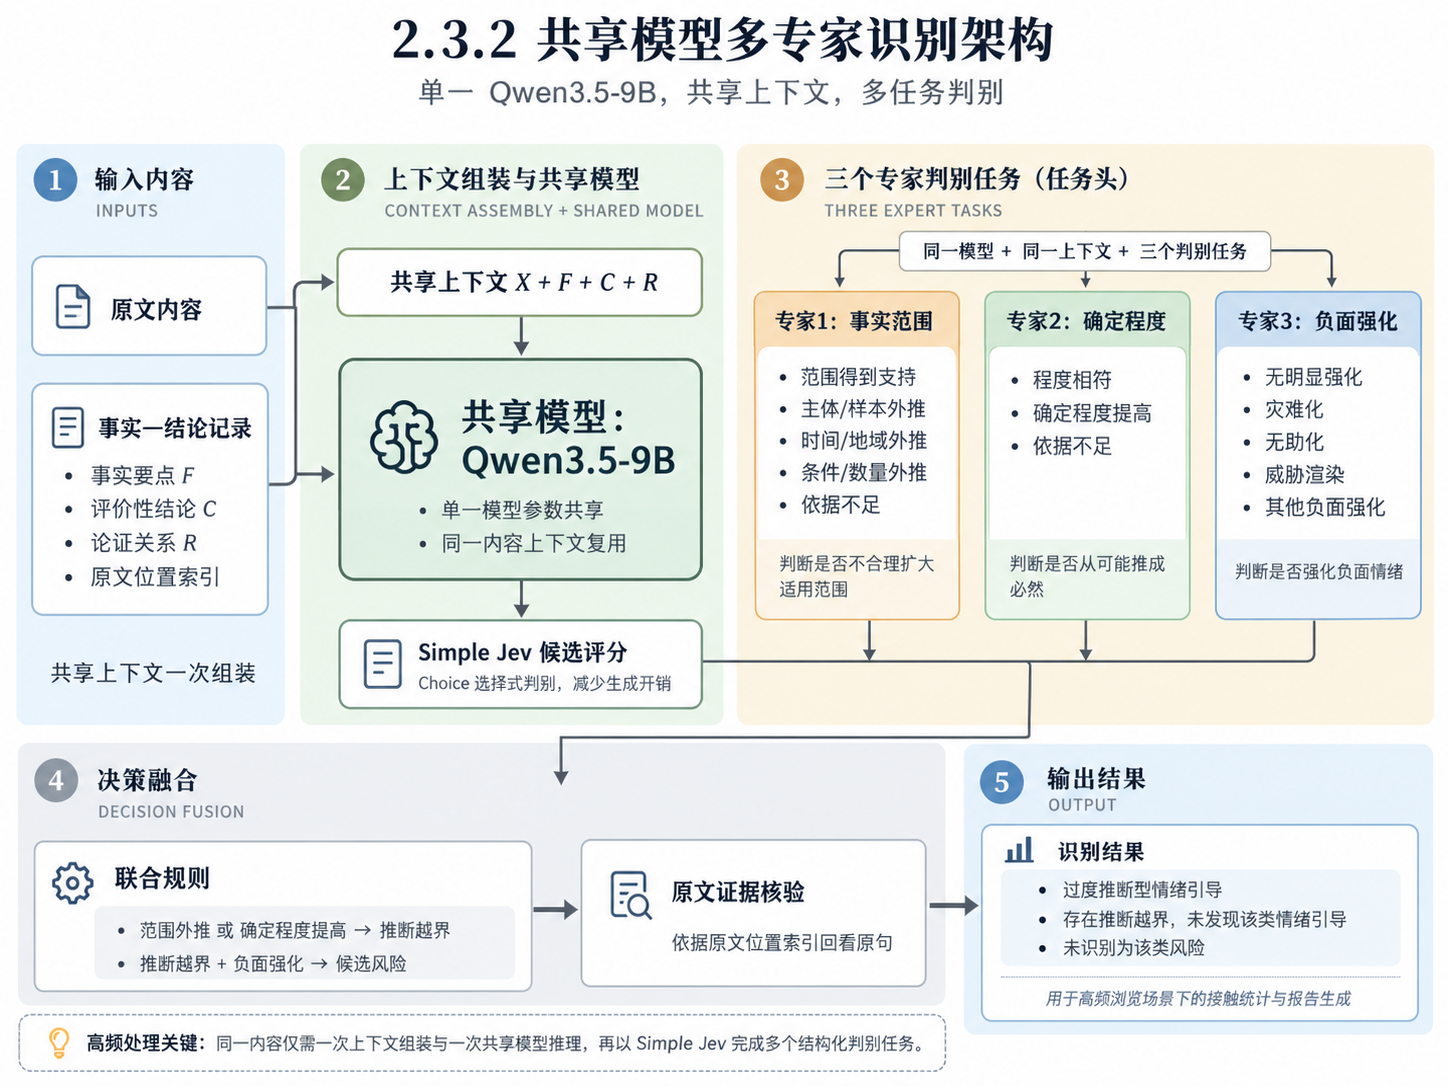
\includegraphics[width=\linewidth,height=0.72\textheight,keepaspectratio]{figures/chapter2/fig_2_4_emotional_guidance.png}
\caption{共享模型多专家识别架构流程图}\label{fig:2-4}
\end{figure}

\subsubsection{基于共享上下文的多专家语义判别}\label{section:2.3.2}

事实外推、确定性提高与负面情绪强化虽然可能同时出现在同一段表述中，但各自对应不同的判断标准。例如，``部分岗位减少''被推及``所有行业''属于事实适用范围的扩大；``岗位可能减少''被改写为``必然失业''则属于结论确定程度的提高。只有将这些差异区分开来，才能说明一条内容的引导性具体来自何处。

据此，系统在Qwen3.5-9B上设置事实范围、确定程度和情绪表达三个语义判别专家。三个专家共享模型参数和内容上下文，分别采用独立的判别问题与候选类别。其中，事实范围专家综合相关事实及其限定条件，识别结论对主体、时间、地域或适用条件的不合理外推；确定程度专家比较事实依据与结论的判断强度，识别从可能、局部到必然、普遍的推断变化；情绪表达专家结合语境，识别灾难化、无助化和威胁渲染等负面强化方式。具体分类设置如下表所示。

\begingroup
\small
\begin{longtable}{@{}
>{\RaggedRight\arraybackslash}p{(\linewidth - 4\tabcolsep) * \real{0.1600}}
>{\RaggedRight\arraybackslash}p{(\linewidth - 4\tabcolsep) * \real{0.2800}}
>{\RaggedRight\arraybackslash}p{(\linewidth - 4\tabcolsep) * \real{0.5600}}@{}}
\caption{三个语义判别专家的分类任务与候选类别}\label{tab:2-2}\tabularnewline
\toprule
判别专家 & 核心判断 & 候选类别 \\
\midrule
\endfirsthead
\toprule
判别专家 & 核心判断 & 候选类别 \\
\midrule
\endhead
\bottomrule
\endlastfoot
事实范围专家 & 结论的适用范围是否获得事实支持 & 范围得到支持；主体或样本外推；时间或地域外推；数量或条件外推；多维外推；依据不足 \\
确定程度专家 & 结论的确定程度是否超出事实依据 & 程度相符；确定程度提高；依据不足 \\
情绪表达专家 & 结论是否采用负面情绪强化表达 & 无明显强化；灾难化；无助化；威胁渲染；其他负面强化；语境不明 \\
\end{longtable}
\endgroup

对于一条包含多项评价性结论的内容，系统将原始文本与2.2节提取的事实、结论和论证关系组成共享上下文，再以结论编号指定各专家的判断对象。Simple Jev将每项判断组织为具有固定候选类别的Choice问题，利用公共输入的计算结果对候选答案进行评分。与逐项生成自然语言解释相比，这种方式将模型推理集中于类别选择，并减少同一内容在多个判断任务中的重复处理。第\(i\)条内容中第\(j\)项结论的专家判别表示为：

\begin{equation}
\hat y_{ij}^{(k)}=\underset{y\in\mathcal Y_k}{\arg\max}\;P_{\theta}\!\left(y\mid X_i,F_i,C_i,R_i,q_{ij}^{(k)}\right),\quad k\in\{\mathrm{scope},\mathrm{certainty},\mathrm{emotion}\}
\label{eq:2-11}
\end{equation}

其中，\(X_i\)为原始内容上下文，\(F_i\)、\(C_i\)和\(R_i\)分别表示事实集合、评价性结论集合及论证关系；\(q_{ij}^{(k)}\)为第\(k\)个专家针对第\(j\)项结论提出的判别问题，\(\mathcal Y_k\)为相应的候选类别集合。\(P_{\theta}\)表示Qwen3.5-9B经Simple Jev计算的候选类别相对得分分布，\(\hat y_{ij}^{(k)}\)为得分最高的类别。三个专家由此获得结构一致、含义互补的判断结果，为后续联合判定提供依据。

\subsubsection{基于逻辑约束的专家决策融合与原文证据核验}\label{section:2.3.3}

三个专家的输出分别描述推断依据与表达方式，仍需进一步确定它们是否共同构成情绪引导。单纯的负面表达可能只是对事实的合理评价；缺乏依据的外推也未必伴随情绪强化。因此，本模块将\textbf{推断越界与负面情绪强化同时出现}作为过度推断型情绪引导的核心判据，并要求相关判断能够对应到原文依据。

具体而言，事实范围专家识别出不合理外推，或确定程度专家识别出缺乏依据的确定性提高时，判定该结论存在推断越界；在此基础上，若情绪表达专家同时识别出负面强化，并通过原文证据核验，则将其归为过度推断型情绪引导。联合判定规则表示为：

\begin{equation}
G_{ij}=\mathbb I\!\left[(S_{ij}\lor D_{ij})\land E_{ij}\land V_{ij}\right]
\label{eq:2-12}
\end{equation}

其中，\(S_{ij}\)和\(D_{ij}\)分别表示事实范围外推与确定程度提高是否成立，\(E_{ij}\)表示是否存在负面情绪强化，\(V_{ij}\)表示原文证据核验是否通过，\(G_{ij}\)为最终判定结果。各类判断组合及其输出如下表所示。

\begingroup
\small
\begin{longtable}{@{}
>{\RaggedRight\arraybackslash}p{(\linewidth - 6\tabcolsep) * \real{0.3100}}
>{\RaggedRight\arraybackslash}p{(\linewidth - 6\tabcolsep) * \real{0.1600}}
>{\RaggedRight\arraybackslash}p{(\linewidth - 6\tabcolsep) * \real{0.1200}}
>{\RaggedRight\arraybackslash}p{(\linewidth - 6\tabcolsep) * \real{0.4100}}@{}}
\caption{多专家决策融合规则}\label{tab:2-3}\tabularnewline
\toprule
推断越界判断 & 负面情绪强化 & 原文核验 & 最终识别结果 \\
\midrule
\endfirsthead
\toprule
推断越界判断 & 负面情绪强化 & 原文核验 & 最终识别结果 \\
\midrule
\endhead
\bottomrule
\endlastfoot
存在范围外推或确定程度提高 & 存在 & 通过 & 过度推断型情绪引导 \\
存在范围外推或确定程度提高 & 未发现 & 通过 & 存在推断越界，未发现该类情绪引导 \\
未发现推断越界 & 存在 & 通过 & 存在负面情绪强化，未发现该类情绪引导 \\
未发现推断越界 & 未发现 & 通过 & 未发现该类情绪引导特征 \\
\end{longtable}
\endgroup

联合判定能否用于认知体检报告，还取决于判断依据是否真实对应用户接触的内容。为此，系统沿用2.2节保存的事实、结论及论据的原文索引，将专家判断关联到具体语句及其所在语境。对于图文内容，索引指向原始文本位置或OCR文字区域；对于视频内容，索引指向语音转写时间戳或画面文字位置。系统据此核对被引用事实的限定条件、事实与结论的论证关系，以及相关表述究竟属于作者自身判断还是对他人观点的转述。

当原文对应关系明确且各项判断一致时，系统形成包含引导类型、推断变化、情绪强化方式和原文位置的识别记录。对于依据不足、语境不明或存在冲突的情况，系统保留待核验状态，并围绕争议结论追加针对性的Jev分类判断。这样，情绪引导标签不仅具有明确的形成规则，也能落实到具体的事实、结论及其来源，为后续报告中的证据展示提供支持。

\subsubsection{用户接触情绪引导内容的统计与展示}\label{section:2.3.4}

对单条结论的判别只能说明某段内容具有什么表达特征，而认知体检还需要回答用户在日常浏览中实际接触了多少此类信息。为此，系统将结论级判断汇总为内容级结果，再与浏览事件中的接触时间、有效停留时长及所属议题关联。当一条内容包含多项结论时，只要其中一项被确认为过度推断型情绪引导，该内容即获得相应标记；同一次浏览始终作为一条事件统计，以保持内容识别和用户接触行为之间的对应关系。

在此基础上，系统计算情绪引导内容在已完成判定浏览事件中的数量占比，以及其有效浏览时长占比，分别反映用户接触此类内容的频率和注意力投入。进一步按照议题和时间窗口汇总，可以识别某一问题下的情绪化推断是否反复出现。例如，用户在一天内连续观看多条将个别裁员事件推断为整体就业危机的视频，报告能够展示这类内容在就业议题中的出现次数、累计浏览时长及主要引导方式。

持续浏览中，同一内容也可能被用户多次观看。系统依据内容标识与原文特征维护语义识别结果，并将其与每次浏览事件分别保存：对于内容未发生变化的重复接触，复用已有判定并记录新的停留信息；对于内容发生变化的情况，则更新相应的语义分析。由此，内容判别服务于信息特征识别，浏览事件记录服务于个人接触统计，两者共同形成长期观察所需的数据基础。

在破茧的个人认知体检报告中，用户既可以通过数量与时长分布了解整体接触情况，也可以进入具体议题查看典型记录。报告同时呈现事实范围变化、结论确定程度变化、负面情绪强化方式及对应的原文片段，使用户能够看到某类信息为何被识别，以及自己在多大程度上接触了这类表达。情绪引导识别由此从孤立的内容标签转化为具有事实依据的个人信息接触分析。

\subsection{基于可验证异构机密计算的全过程隐私保护方法}\label{section:2.4}

\subsubsection{隐私保护目标与泄露风险}\label{section:2.4.1}

破茧需要持续分析用户接触的屏幕内容、可采集音频及浏览行为，并由此形成议题、观点、论据和情绪引导等长期记录。这些信息不仅可能涉及某次浏览中的私人内容，还能反映用户长期的关注方向与信息接触习惯。因此，破茧将隐私保护目标明确为：\textbf{用户浏览内容及其敏感分析结果，只在用户手机和经过验证的可信计算环境内以明文出现；普通服务器可以管理任务和资源，却不能仅凭管理权限获得数据解密权。} 系统的隐私保护不依赖服务器被善意管理，而依赖可核验的技术约束。

实现这一目标的难点在于，OCR、语音转写和大模型推理必须读取明文。常规通信加密能保护上传途中的数据，数据库加密能保护静态文件，却不能阻止服务器在解密后读取内存，或把数据交给未经认可的程序。破茧因此采用\textbf{可验证异构机密计算}方案：``可验证''是指手机通过远程证明核验云端实际运行的环境和程序身份，验证成功后才交付解密权限；``异构''是指CPU和GPU共同处理敏感数据，两侧的内存及传输链路都纳入硬件保护范围。对应采用四项措施：通过开源审计与版本验证约束客户端的数据采集行为、验证云端可信程序后才允许加密上传、使用TDX与机密GPU保护运行中的明文，以及由用户保管长期密钥并加密保存历史。四项措施分别针对一条主要泄露途径，见表~\ref{tab:2-4}。

\begingroup
\small
\begin{longtable}{@{}
>{\RaggedRight\arraybackslash}p{(\linewidth - 6\tabcolsep) * \real{0.2200}}
>{\RaggedRight\arraybackslash}p{(\linewidth - 6\tabcolsep) * \real{0.3600}}
>{\RaggedRight\arraybackslash}p{(\linewidth - 6\tabcolsep) * \real{0.3000}}
>{\RaggedRight\arraybackslash}p{(\linewidth - 6\tabcolsep) * \real{0.1200}}@{}}
\caption{破茧全过程隐私泄露途径与防护措施}\label{tab:2-4}\tabularnewline
\toprule
可能的泄露途径 & 如何阻止泄露 & 关键技术 & 对应小节 \\
\midrule
\endfirsthead
\toprule
可能的泄露途径 & 如何阻止泄露 & 关键技术 & 对应小节 \\
\midrule
\endhead
\bottomrule
\endlastfoot
手机客户端超范围采集，或通过恶意程序外传原始内容 & 公开客户端的数据采集和通信代码，接受安全审计，并通过构建验证和版本审核确保实际发布的程序与审核版本一致 & 开源代码审计、可复现构建、多方签名、Android系统授权 & 2.4.2 \\
上传数据被截获，或被转交给替换后的解密程序 & 手机先核验实际运行的程序和本次接收公钥，确认后才加密发送；传输过程安全由机密计算服务器提供保障 & 可信版本清单、UKI、dm-verity、TDX与GPU远程证明、HPKE & 2.4.3 \\
OCR及模型推理期间，内存、显存或日志暴露明文 & 明文仅在受保护的CPU和GPU中处理，设备间传输加密，由机密计算服务器提供安全保障；可信程序限制调试、日志与对外通信 & Intel TDX、NVIDIA GPU机密计算、受保护的CPU---GPU通道 & 2.4.4 \\
数据库或备份中的历史索引、分析报告被下载并还原 & 手机保管长期主密钥，仅按次向可信程序提供本次所需的数据密钥；运营服务器存储端只保存密文，无法获取明文信息 & Android Keystore、AES-256-GCM、按次密钥授权与历史版本校验 & 2.4.5 \\
\end{longtable}
\endgroup

上述保护以用户手机及其运行的授权客户端、可信程序的审核与版本批准机制，以及CPU、GPU硬件和远程证明体系可信为前提。普通业务服务器仍可获知任务发生时间、密文大小等必要通信元数据，但不能据此直接读取浏览正文或个人语义记录。

\begin{figure}[htbp]
\centering
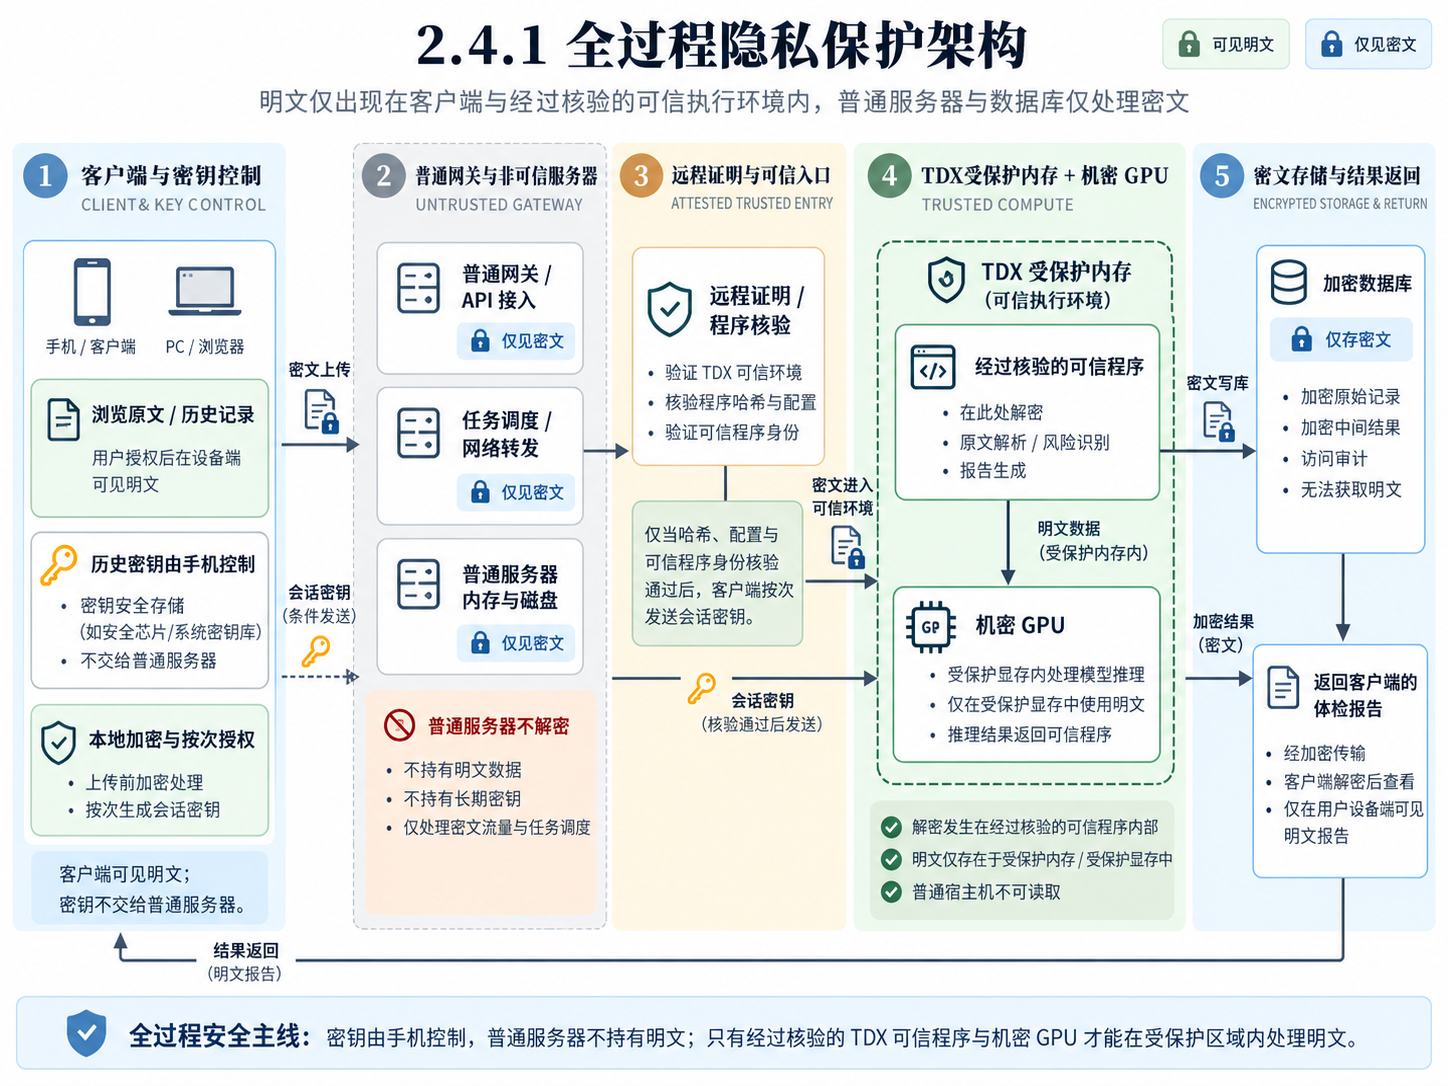
\includegraphics[width=\linewidth,height=0.72\textheight,keepaspectratio]{figures/chapter2/fig_2_5_privacy_protection.png}
\caption{全流程隐私保护架构}\label{fig:2-5}
\end{figure}

\subsubsection{防止原始内容在手机采集阶段泄露}\label{section:2.4.2}

用户的截图、音频及浏览行为首先由手机客户端采集，因此客户端本身构成隐私保护的第一道关口。即使用户已通过系统权限弹窗授权采集，也无法据此判断软件是否存在超范围记录、私自保存或向外部服务器发送数据的逻辑。一旦客户端程序存在恶意行为，后续的传输加密与云端机密计算都无法阻止原始数据泄露。因此，\textbf{手机端隐私保护的关键不仅是限制采集权限，更要保证客户端执行的是经过审查的可信程序。}

针对这一风险，破茧采用开源与安全审计相结合的程序验证机制。系统公开屏幕采集、音频处理、数据暂存及网络通信等安全关键代码，使用户及第三方能够检查数据获取范围与对外传输行为。同时，系统提供可复现构建信息，将公开源代码与实际发布的安装包建立对应关系。正式版本采用多方签名批准策略，并预留独立审核方参与审计的机制，防止未经认可的代码修改直接进入受信任的客户端版本。通过代码行为审查与发布版本验证，降低客户端利用采集权限私自获取或外传用户信息的风险。

在实际采集过程中，破茧通过Android MediaProjection获取用户授权的屏幕画面，按照端侧采样和区域裁剪规则保留必要内容，并仅在系统允许时获取音频。采集结果在应用受控内存中处理，不写入公共相册或明文日志；需要本地暂存时，采用由Android Keystore保护的密钥进行加密。由此，开源审计与版本控制约束客户端程序行为，操作系统授权限定数据获取权限，本地加密则保护必要的暂存记录。

\subsubsection{防止数据被交给未经认可的程序}\label{section:2.4.3}

上传阶段存在两条直接的泄露路径：一是通信中间节点截获数据，二是接收方被冒充。例如，服务器可以返回一把由自己掌握的公钥，让手机误以为它属于可信程序。即使云端启用了可信执行环境（TEE，即受硬件隔离的计算区域），未经审查的程序仍可能在其中解密数据并主动外传。因此，破茧需要同时验证\textbf{程序版本是否获准}与\textbf{本次加密公钥是否确实属于该程序所在的可信环境}。

与手机端的程序审核相对应，系统公开服务端的解密、模型调用、历史读写和通信等安全关键代码，固定正式版本的依赖、模型文件和安全配置，并提供可复现构建信息，使公开源码与发布产物能够对应。受认可的版本写入可信版本清单。清单采用多方签名批准策略，并预留独立审核方参与审核和签名的接口，普通业务后台不能自行增加可信版本。云端使用统一内核映像（UKI）将内核和启动配置纳入完整性测量，使用\texttt{dm-verity}校验只读系统文件，进而把允许执行的工作负载与可信启动状态对应起来。手机检查的不是服务器自行声称的代码哈希，而是硬件远程证明中记录的实际运行度量是否符合已批准清单。

在此基础上，破茧按以下步骤建立数据传输会话：

\begin{enumerate}
\def\labelenumi{\arabic{enumi}.}
\setlength{\itemsep}{0pt}\setlength{\parskip}{0pt}
\item
  \textbf{手机发出核验请求。} 客户端生成一次性随机数，要求云端提供本次运行环境的证明。可信程序在受保护的CPU内存中生成临时公私钥，私钥不交给普通网关。
\item
  \textbf{云端出具硬件证明。} Intel TDX提供可信虚拟机的启动状态和运行度量证明，NVIDIA提供GPU机密计算状态的证明。可信程序把手机随机数、临时公钥和GPU证明摘要组合成绑定值，写入TDX证明中的\texttt{REPORTDATA}字段。该字段用于证明这份材料对应的是\textbf{本次请求和本次公钥}。
\item
  \textbf{手机独立核验。} 客户端验证两类硬件证明的真实性与安全状态，核对可信虚拟机的度量值是否符合已批准版本，并检查随机数、公钥及GPU证明的绑定关系。可信程序还核对被证明的GPU就是实际承担推理的设备。任何一项不符合要求，客户端都不发送浏览内容或解密密钥。
\item
  \textbf{验证成功后加密上传。} 客户端采用HPKE（一种基于接收方公钥建立加密会话的标准机制）加密截图、音频及浏览事件。普通API网关只负责转发密文，无法凭转发权限还原数据。
\item
  \textbf{可信程序在内部解密。} 密文到达可信虚拟机后，由持有临时私钥的破茧接收程序在受保护的CPU内存中解密，再交给后续模型处理。解密不经过普通业务服务器，也不由云平台管理控制台执行。
\end{enumerate}

TDX远程证明直接反映的是虚拟机状态，并不会自动证明任意应用进程都可信。因此，系统将固定工作负载、受验证启动、程序访问权限和会话密钥绑定共同纳入准入条件，使获得解密权限的对象对应到批准的接收程序。这样，运营方即使能够转发请求、管理实例，也不能仅靠更换程序或公钥取得用户明文。

\subsubsection{防止明文在CPU与GPU计算期间泄露}\label{section:2.4.4}

数据进入可信程序后必须暂时解密，否则OCR无法读取像素，语义模型也无法理解文本。此时的风险不再是网络窃听，而是计算设备本身：普通云服务器的管理权限可能触及进程内存，模型推理还会使数据进入GPU显存。如果只保护CPU而不保护GPU，明文仍可能在显卡或两者之间的传输过程中暴露。

破茧采用阿里云\texttt{ecs.gn8v-tee.4xlarge}异构机密计算实例。Intel TDX为可信虚拟机提供CPU内存隔离，限制宿主机及虚拟化管理层对受保护数据的访问；NVIDIA GPU机密计算保护GPU中的敏感数据。可信虚拟机内的GPU驱动与显卡建立受保护的通信通道，使CPU与GPU之间传递的模型输入和中间结果在设备传输链路上保持加密状态。云平台提供上述硬件能力，破茧负责把自身的解密、OCR、语音转写和语义分析程序放入同一受保护的工作负载中。

解密后的截图和音频先在受保护的CPU内存中完成解码与时间对齐，再送入可信GPU进行OCR、语音转写和模型推理。2.2节的议题、观点和论据分析，以及2.3节的情绪引导识别，都在该计算边界内部进行；BM25检索、历史比较、指标统计和加密写回等操作由可信虚拟机内的CPU程序处理。用户原文、语义向量和提示词不交给外部在线模型接口，也不返回普通业务服务进行二次处理。

硬件隔离还需要与程序输出限制配合。正式可信工作负载不开放用于读取明文的远程登录与调试接口，关闭明文业务日志和内存转储，并限制未经批准的网络出口及运行时程序加载。这些限制作为可信版本配置的一部分接受完整性验证，避免程序把受保护环境内的内容通过正常输出通道带出。由此，\textbf{明文只为必要的OCR和模型推理在可信CPU内存与GPU显存中短暂存在，不因服务器的日常管理操作而对外暴露。}

\subsubsection{防止历史数据与报告在长期存储中泄露}\label{section:2.4.5}

单次计算结束后，破茧还需保存用户接触过的议题、观点、事实要点和情绪统计，以支持后续比较与认知体检。即使删除原始截图，BM25索引、语义向量和分析报告仍可能反推出用户关注的具体内容。如果数据库存储着可直接解密这些记录的密钥，前面建立的计算保护便会在长期存储阶段失效。

破茧将长期主密钥保留在用户手机，并通过Android Keystore进行本地保护。用户的浏览事件、议题和观点簇、事实要点、检索索引及认知体检报告，均使用用户控制的数据密钥进行AES-256-GCM认证加密，再写入普通数据库。数据库只保存密文与必要的记录标识，不保存长期主密钥。数据库管理者可以备份、迁移或删除记录，但不能仅凭数据库权限恢复其中的浏览内容。

当新内容需要与历史比较时，手机再次核验可信程序，\textbf{按次交付完成本次分析所需的数据密钥，用后销毁，长期主密钥始终留在手机}。可信程序在受保护内存中解密所需的历史索引，完成候选检索、全局或相关历史比较以及索引更新，并将更新结果重新加密写回。是否需要检索全部历史由2.2节的分析任务决定；无论读取范围如何，解密与检索均在可信环境内执行，而不是要求普通数据库直接查询明文。分析报告同样以密文存储，或经过本次受保护会话返回手机供用户查看。

AES-256-GCM能够检测密文被篡改，但单靠它无法识别数据库故意返回一个完整的旧版本。因此，系统还为历史状态维护版本号和完整性摘要，并由客户端保存最近确认的状态标识，核对后续读取与更新结果的连续性。会话结束时，可信程序清除临时密钥与可访问的明文缓存；没有新的用户授权，服务器不能自行恢复历史记录开展额外计算。

至此，破茧沿数据处理过程封闭了四类主要泄露途径：在手机端通过代码审核与版本验证约束采集行为，在上传前核验解密接收方，在CPU与GPU运行期间隔离明文，并在长期存储时把解密权保留给用户。\textbf{保护机制的核心不是要求服务器管理者始终可信，而是使其管理权限不足以直接取得用户的浏览明文和长期分析结果。}

\subsection{认知体检报告生成与主动反馈机制}\label{section:2.5}

前述信息茧房识别与情绪引导识别方法，已经能够对单条浏览内容及其历史关系作出判断，但用户最终需要了解的并非某条记录的分类结果，而是自己在一段时间内接触了哪些信息、哪些判断依据不断重复，以及是否存在值得进一步查证的内容。为此，破茧将浏览事件与议题、观点、论据和情绪引导记录关联，在已有分析结果的基础上生成分时段认知体检报告，并通过主题整理、信息盲区提示和主动提醒，将识别结果转化为用户可以理解和自主使用的信息。

\subsubsection{多维认知指标的汇总与报告生成}\label{section:2.5.1}

认知体检报告首先需要解决不同分析结果难以直接比较的问题。浏览时长描述用户的注意力投入，观点分布反映所接触的判断结构，信息增量说明新增了多少事实依据，情绪引导识别则刻画部分内容的推断与表达特征。如果将这些结果分别展示，用户仍然难以判断某个时段究竟因何形成较高的信息重复或情绪引导接触比例。因此，系统以浏览事件为共同时间索引，将2.2节和2.3节的分析结果统一组织到``时间窗口---议题---具体内容''的统计层次中。

系统分别维护浏览事件、浏览内容和事实依据三种统计口径。接触次数与有效浏览时长依据浏览事件计算，同一视频被反复观看时保留每次接触；已浏览内容数量依据内容标识去重，反映用户实际看过多少条不同材料；去重论据数量则根据2.2.3节的事实等价与联合覆盖结果计算，避免将多条视频重复引用的同一事实视为多项独立依据。每条记录通过内容标识、议题标识、观点簇及原文索引建立关联。一条内容涉及多个议题时，可以分别进入相应议题的分析，但总体浏览次数仍按原始事件计算，避免跨议题重复累加。

在时间组织上，系统形成小时、每日和长期三个层次的认知体检报告。小时报告以24小时浏览分布图展示一天内各时段的有效浏览时长及主要议题，用户进入某个时段后，可以查看该时段涉及的观点和内容构成。浏览事件按实际接触时间归属，跨越小时边界的有效浏览时长按对应时段分配。每日报告进一步汇总各议题的浏览内容数量、有效接触时长、观点分布、去重论据数量和信息增量率，并展示过度推断型情绪引导内容的接触次数及其时长占比，使浏览投入与实际获得的信息能够在同一议题下对照查看。

对于用户持续关注的议题，系统直接复用2.2.4节定义的观点集中度、有效观点数量、去重论据数量和信息增量率，形成可比较的时间序列。长期报告按连续有效窗口观察这些指标的变化，并呈现2.2.5节的信息茧房风险判定结果。例如，某议题的浏览时长连续增加，但主要观点始终集中于同一判断，信息增量率持续较低，报告便能够同时展示``投入时间增加''和``新增依据不足''两个现象及其历史变化。情绪引导统计则采用2.3.4节的内容级识别结果，以已完成判定的浏览事件为分母计算接触比例，避免将待核验内容直接计入已确认的情绪引导记录。

报告采用基于结构化记录的增量汇总方式。每次授权分析完成后，系统将新的浏览事件及其判别结果写入相应时间和议题的统计记录，无需为生成报告重复执行全文观点抽取或情绪识别。当历史议题归并、观点簇调整或论据覆盖关系得到修正时，系统依据原有事件关联重新计算受影响的统计结果。对于采集覆盖不足、有效记录过少或判断尚未完成的窗口，报告标明相应的数据范围，并保留风险判定中的证据不足状态。最终形成的统计结果按2.4节的机制加密保存，在用户授权的可信会话中更新，并返回手机供其查看。

\subsubsection{基于原文溯源的主题观点整理}\label{section:2.5.2}

时间分布与风险指标能够说明用户近期的信息接触特征，却无法代替对具体内容的回顾。尤其在短视频和社交平台中，同一问题的相关材料常常分散在不连续的浏览时段，中间穿插大量无关内容。用户即使接触过不同观点，也很难回忆它们分别来自哪些视频，又获得了什么事实支持。为此，破茧利用2.2节已经建立的议题档案、观点簇和论据关系，将分散的浏览内容整理为可追溯的主题观点卡片。

观点卡片以议题为入口，以已归并的观点簇为整理单位。系统首先按照用户选择的日期或历史范围，检索该议题下已经接触的观点记录，再依据2.2.2节确定的表达主体和支持、反驳关系，将真正支持某一观点的内容关联到对应卡片。被作者引用后加以反驳的观点，不计入作者支持该观点的内容数量。卡片使用2.2.3节维护的观点簇名称，展示观点的主要判断、支持它的已浏览内容数量，以及与其他观点存在的分歧关系，使用户能够直接比较同一问题下实际接触到的不同说法。

在每张卡片内部，系统进一步按照事实要点及其适用条件整理关联论据，并合并语义等价的重复依据。每项论据保留支持或反驳关系，同时展示它被多少条不同的已浏览内容引用，以及这些内容对应的原始来源。例如，十条就业视频都支持``招聘形势严峻''，但其中八条引用同一份裁员报道，卡片将分别呈现支持该观点的内容数量与去重后的论据，避免用户将多次传播误认为多项独立证据。对于能够由不同历史材料共同覆盖的复合论据，系统沿用已有事实要点关联，而不把重新组合的表述直接认定为新增事实。

观点及论据的展示内容均与原文索引建立对应关系。用户点击具体论据后，可以查看被引用的事实片段、相关观点语句及其上下文，并根据已保存的来源标识定位原网页位置或视频转写时间点。对于能够重新访问的原始内容，系统提供来源入口；对于暂时无法打开的来源，仍可查看授权分析过程中保存的相关文本片段及其出处信息。这样，主题总结不仅说明``用户看到了哪些观点''，还能够回答``这些观点由哪些材料支持''，使其成为可以反复核查的个人信息整理结果。

随着后续浏览增加，新的内容继续归入对应议题和观点簇，卡片中的关联内容、论据数量与来源记录同步更新。若历史比较确认议题或观点簇需要合并，系统按照2.2.3节的标识映射调整卡片关联，而不丢失原始来源。用户由此可以跨越不同日期持续回顾同一个问题，也能够根据卡片中呈现的观点分布与证据重复关系，发现已有信息尚未充分覆盖的部分。

\subsubsection{信息盲区提示与信息补全}\label{section:2.5.3}

观点整理让用户看到已经获得的材料，但当某一议题长期由少数观点主导时，用户更关心的是还需要了解什么。仅给出``观点集中度较高''的数值，并不能指出下一步应补充哪些信息。另一方面，个人浏览记录只能反映用户实际接触的内容，不能直接证明未出现的观点一定存在，或判定某种相反说法必然正确。因此，破茧将信息盲区提示建立在\textbf{已有浏览材料的覆盖范围}之上，重点指出当前认识所依赖的观点、事实条件及来源可能存在哪些局限。

系统首先利用2.2节形成的议题历史，比较近期窗口与较长历史范围内的观点簇和论据记录。如果某种观点曾在历史中出现、近期却很少接触，系统可以提示用户回顾该观点及原有依据；如果近期大量内容表达相似判断，而去重论据数量有限、信息增量率持续较低，则提示用户当前接触的材料主要重复了哪些事实。系统还利用事实要点中的主体、时间和地域等限定条件，归纳浏览材料实际覆盖的范围。例如，用户近期关于就业的内容主要涉及互联网企业裁员，提示便指出当前材料集中于该行业和相关事件，而不据此推断整个就业市场均呈现相同情况。

这些提示优先利用已经保存的历史记录完成。对于历史中存在的不同观点或尚未在近期出现的事实依据，系统直接关联对应的观点卡片与原文来源，帮助用户重新查看已有信息；对于历史中尚未出现的观点或事实，系统只说明``当前已浏览材料尚未覆盖''，并给出可进一步查证的方向。信息盲区由此表现为个人接触记录中的覆盖不足，而不是系统凭空生成的相反立场。

当个人历史无法提供足够的补充材料时，用户可以自主发起外部资料检索。系统根据当前议题名称及需要补充的事实维度，形成不包含个人浏览原文和行为记录的通用检索词，由用户确认后通过手机端发起查询。对于就业议题，补充方向可以是其他行业的招聘数据、不同地区的就业统计，或相关调查报告的原始出处。检索结果按照发布时间、来源及事实适用条件展示，重点寻找能够增加独立依据或扩展观察范围的材料，而不是机械推荐与现有观点相反的内容。

用户选择进一步分析外部资料时，候选文本可以经重新核验的加密会话进入可信计算环境，复用2.2节的议题匹配与论据比较方法，检查它相对于个人历史是否提供了新的事实要点。外部检索结果在用户实际阅读前，仅作为待查看的补充资料，不计入已浏览内容数量及信息增量率。该功能采用用户按需发起的方式，不依赖持续的外部网络检索；客户端同时向用户说明，外部检索服务可能获知其主动提交的查询词，用户可以修改关键词或完全不使用此功能。通过区分已有历史回顾与外部资料补充，系统既能够指出信息覆盖不足，也将是否扩展信息来源的决定权交给用户。

\subsubsection{风险提醒与用户自主交互}\label{section:2.5.4}

认知体检报告主要支持用户主动回顾，但观点长期集中或过度推断型情绪引导反复出现时，用户未必会及时打开报告。为使长期分析结果能够在需要时发挥作用，破茧将已经完成核验的风险记录转换为可查看依据的提醒，并通过用户设置控制提醒时机与频率。提醒的目标是提示当前浏览材料值得复核，而不是替代用户判断内容是否真实，或推断用户已经产生了某种情绪变化。

信息茧房提醒直接以2.2.5节的长期风险判定为依据。当某个议题在足够数量的有效窗口中持续满足观点集中与信息增量不足的联合条件，且风险状态为触发预警时，系统生成对应提示；处于证据不足状态的议题不触发该类预警。情绪引导提醒则使用2.3节已经完成原文核验的内容级结果：当预设时间窗口内此类内容达到最低接触次数，且其数量占比或有效浏览时长占比达到提醒阈值时，系统才生成相应提示。两类提醒分别依据长期信息重复模式和已确认的过度推断型情绪引导接触情况，不将单次浏览或普通负面信息直接视为风险。

提醒内容由可信计算环境依据风险类型及关联原文记录形成，通过受保护会话交付手机客户端，由手机本地展示通知。通知首页仅使用简要、非敏感的提示文字，具体议题、观点和浏览内容在用户打开应用后展示，避免通过普通推送服务暴露个人关注的问题。由于2.4节的历史解密机制依赖用户按次授权，系统只针对已获授权并完成分析的记录更新提醒；没有有效授权会话时，云端不自行解密历史数据进行后台扫描，后续提醒在客户端下一次获得相应分析结果时合并呈现。

为减少持续信息流中的重复打扰，系统按照议题和提醒类型维护通知状态。同一议题的相同风险在设定的间隔内只提示一次；若风险条件仍然持续，但没有出现新的实质性依据，则合并进入每日报告，不反复推送。多个相关记录在短时间内触发时，系统优先合并为一条汇总提醒。用户可以选择仅接收每日摘要、设置免打扰时段、调整提醒频率，也可以关闭特定议题或某类风险的通知，使认知安全提示服从实际使用需要。

用户打开提醒后，系统提供从结论返回依据的查看路径。对于信息茧房提醒，页面展示对应时间窗口的主导观点比例、信息增量变化，以及反复出现的事实要点与来源；对于情绪引导提醒，页面展示原文中被引用的事实、相关结论及识别出的范围外推或确定程度提高，并标明负面强化方式。用户可以进入相应观点卡片查看完整上下文，也可以对议题归属、观点归并或原文对应关系提出纠正。涉及分析记录的修正由后续授权的可信程序重新核验，并更新受影响的统计结果与提醒状态。

通过以上机制，破茧将连续浏览产生的内容分析结果组织为可回顾、可追溯的认知体检报告，再由报告中的观点与论据关系发现信息覆盖局限，并在长期风险成立时提供适度提醒。用户能够据此回顾实际获得的判断依据，自主选择是否查阅补充资料，以及如何接收和使用提示，使个人认知安全防护与日常信息管理形成连续的使用过程。
